\section{Contexto y motivaci\'on}

Los mercados financieros generan registros temporales abundantes y heterog\'eneos.
Un mismo activo puede analizarse combinando velas intradiarias,
datos diarios, niveles t\'ecnicos, indicadores de momento, correlaciones con
otros activos e informaci\'on externa de contexto. Esta variedad de fuentes puede
ser \'util para quien revisa posibles compras y ventas en activos financieros,
pero tambi\'en plantea un problema de integraci\'on, filtrado y priorizaci\'on de
datos. Aumenta el tiempo necesario para analizar cada activo y dificulta
mantener una visi\'on ordenada de los candidatos de an\'alisis.

En el an\'alisis t\'ecnico es frecuente trabajar con reglas visuales o
semidiscrecionales, es decir, reglas que combinan criterios definidos con
interpretaci\'on humana: rupturas, retrocesos, cruces de indicadores, zonas de
soporte y resistencia o estructuras de impulso y correcci\'on. Muchas de estas
ideas se explican de forma intuitiva y se aplican mediante criterio humano,
pero no siempre quedan expresadas como reglas que puedan comprobarse de manera
sistem\'atica. Esta diferencia es importante, porque una idea que parece
razonable en un gr\'afico concreto puede comportarse de forma distinta cuando se
eval\'ua sobre muchos activos, periodos y configuraciones.

La motivaci\'on de este Trabajo de Fin de Grado surge de esa necesidad de ordenar el
proceso. El prop\'osito no es sustituir el criterio del usuario. Se busca construir
una base que reduzca la carga y el tiempo de revisi\'on inicial, priorice
candidatos de estudio y conserve evidencias revisables. Tambi\'en se separa de forma expl\'icita
la observaci\'on del mercado de cualquier paso operativo. En lugar de tratar una
se\~nal aislada como una decisi\'on final, el trabajo plantea un flujo en el que
las reglas se formalizan, se eval\'uan y se presentan junto con su contexto.

\section{Antecedentes}

El trabajo se apoya en dos familias de ideas. La primera procede del an\'alisis
t\'ecnico cl\'asico. En esta l\'inea se utilizan indicadores como el \'indice de fuerza relativa
(RSI), la convergencia/divergencia de medias m\'oviles (MACD), medias m\'oviles,
bandas de Bollinger o niveles de Fibonacci. Sirven para describir situaciones
de mercado y plantear reglas de entrada o salida \cite{murphy_1999_technical_analysis,wilder_1978_new_concepts,appel_2005_power_tools,bollinger_2001_bands}.
Estas herramientas no son, por s\'i solas, una garant\'ia de rentabilidad, pero
ofrecen un lenguaje com\'un para transformar observaciones visuales en
condiciones calculables. La forma concreta en que estos indicadores intervienen
en las reglas del TFG se desarrolla en el cap\'itulo metodol\'ogico, cuando se
explican los setups formalizados y las m\'etricas de evaluaci\'on.

La segunda familia de ideas est\'a relacionada con la teor\'ia de las ondas de
Elliott y la interpretaci\'on de estructuras de impulso y correcci\'on
\cite{frost_prechter_1985_elliott,balan_1989_elliott_fx,menendez_larre_2016_ondas}.
Esta lectura se conecta, adem\'as, con la idea de que los precios pueden mostrar
comportamientos de escala y cierta estructura fractal
\cite{mandelbrot_1963_speculative_prices,mandelbrot_hudson_2004_misbehavior}.
En este contexto, el enfoque de Men\'endez se toma como referencia metodol\'ogica
para estudiar c\'omo una lectura visual de ondas puede traducirse a criterios
m\'as concretos. A partir de esa referencia se construyen reglas propias,
nombradas seg\'un la condici\'on t\'ecnica que representan, y se separan
\textit{setup}, entendido como configuraci\'on candidata de estudio, contexto,
se\~nal de estudio y posible ejecuci\'on.

Desde una perspectiva econ\'omica, el inter\'es de estudiar estructuras temporales
del precio no depende \'unicamente de aceptar la teor\'ia de Elliott como marco
interpretativo. En los mercados financieros, una noticia, un cambio de
expectativas o una presi\'on compradora o vendedora puede transmitirse de forma
gradual, a medida que distintos participantes incorporan esa informaci\'on o
reaccionan a la evoluci\'on del propio precio. Esta continuidad puede entenderse
como una forma de persistencia temporal o \textit{momentum}
\cite{jegadeesh_titman_1993_momentum}, sin asumir por ello que el mercado sea
f\'acilmente predecible. Aun as\'i, justifica estudiar si algunos movimientos
presentan estructura suficiente como para ser descritos, medidos y comparados.

Desde esta perspectiva, Elliott y el enfoque de Men\'endez Larre se utilizan en
este trabajo como una forma concreta de organizar hip\'otesis sobre impulsos,
correcciones y repeticiones de estructura en distintas escalas temporales. Esta
lectura resulta especialmente \'util porque conecta la interpretaci\'on visual de
las ondas con la idea de fractalidad temporal, pero obliga tambi\'en a formalizar
con cuidado qu\'e se considera \textit{setup}, qu\'e se considera contexto y qu\'e se
eval\'ua como se\~nal de estudio. La memoria no pretende identificar las causas
econ\'omicas \'ultimas de cada movimiento ni demostrar una ley universal del
mercado. El objetivo es m\'as acotado: traducir una lectura t\'ecnica basada en
estructura temporal a reglas computables, compararlas con referencias y analizar
si aportan evidencia \'util dentro del escenario estudiado.

Tambi\'en resulta necesario considerar la evaluaci\'on de estrategias de trading,
entendidas como reglas de compra y venta sobre activos financieros, con cautela.
Un backtest permite estudiar el comportamiento hist\'orico de una regla. Sin
embargo, puede inducir conclusiones demasiado optimistas si no se controlan
problemas como el sobreajuste, el uso de informaci\'on futura o una lectura
incorrecta de los costes y supuestos de ejecuci\'on
\cite{pardo_2008_trading_strategies,bailey_etal_2017_backtest_overfitting,lopez_de_prado_2018_afml}.
Por ello, en esta memoria el backtesting se interpreta como una herramienta de
an\'alisis, no como una demostraci\'on directa de que una estrategia vaya a ser
rentable en condiciones reales.

\section{Problema abordado}

El problema central del TFG es convertir un proceso de revisi\'on disperso y en
parte subjetivo en un flujo m\'as ordenado, trazable y evaluable. En la pr\'actica,
una estrategia puede depender de varios elementos: una condici\'on principal, un
contexto de tendencia, un nivel t\'ecnico, una confirmaci\'on de ruptura, una
estructura de ondas o una restricci\'on de riesgo. Si todos esos elementos no se
separan con claridad, resulta dif\'icil saber qu\'e se est\'a evaluando realmente.
Esto es especialmente relevante en las lecturas basadas en Ondas de Elliott,
porque un mismo tramo de precio puede admitir varios conteos razonables de
impulso y correcci\'on. Por ello, el trabajo no parte de un conteo \'unico y
evidente, sino de la necesidad de transformar hip\'otesis visuales en criterios
revisables.

A partir de ese problema aparecen dos necesidades complementarias. La primera
es cuantitativa: las reglas deben expresarse con suficiente precisi\'on para
probarlas, compararlas y revisar sus supuestos sin introducir informaci\'on
futura. La segunda es interpretativa: el sistema debe presentar el contexto del
mercado de forma comprensible, sin convertir cada hip\'otesis t\'ecnica en una
decisi\'on operativa. El trabajo aborda estas necesidades mediante una
combinaci\'on de formalizaci\'on de reglas, benchmarks, an\'alisis estructural,
dashboard y auditor\'ia de decisiones.

La gesti\'on del riesgo tambi\'en forma parte de ese problema de separaci\'on. No
basta con detectar una posible entrada; el sistema debe diferenciar entre un
caso que solo merece revisi\'on, una propuesta que puede auditarse con reglas de
control y una acci\'on limitada a una demostraci\'on controlada. En ese contexto,
las correlaciones y las comprobaciones previas sirven para advertir posibles
concentraciones de riesgo, pero no sustituyen a una gesti\'on integral de cartera.

El problema tambi\'en incluye la gesti\'on del l\'imite operativo. Cuando el sistema
se conecta con herramientas externas, deja de ser suficiente calcular una
se\~nal: hay que definir qu\'e capas pueden actuar, cu\'ales solo informan y qu\'e
queda fuera del alcance. Bajo ese criterio, una plataforma de apoyo al an\'alisis
puede aportar valor sin convertirse en un sistema aut\'onomo de trading.

\section{Objetivos del trabajo}
\label{sec:objetivos-trabajo}

\subsection{Objetivo general}

El objetivo general de este Trabajo de Fin de Grado consiste en construir una
plataforma de visualizaci\'on y apoyo al an\'alisis de estrategias de trading.
Esta plataforma busca ordenar el an\'alisis del mercado a partir de datos,
reducir el tiempo dedicado a tareas repetitivas de revisi\'on, priorizar
candidatos de estudio y mantener una visi\'on
ordenada de la informaci\'on disponible. El prop\'osito no es sustituir el
criterio del usuario ni desarrollar un sistema que opere de forma totalmente
aut\'onoma. Se busca crear una base t\'ecnica que permita estudiar reglas de
entrada, contextualizarlas con datos de mercado, aprovechar mejor la evidencia
disponible y presentarla de forma clara para facilitar la toma de decisiones
supervisada.

Para ello, el trabajo busca convertir estrategias y criterios originalmente
descritos de forma discrecional en reglas que puedan calcularse, compararse y
evaluarse de manera sistem\'atica mediante distintos m\'etodos. Esta
formalizaci\'on se basa en datos intradiarios y diarios. Adem\'as, se apoya en
informaci\'on externa de contexto cuando procede, en procesos de backtesting y
en la comparaci\'on con estrategias de referencia. De este modo, la evaluaci\'on
de cada estrategia no se apoya solo en la lectura puntual de una se\~nal. Tambi\'en
se apoya en un conjunto de evidencias revisables: m\'etricas de comportamiento,
tablas comparativas, gr\'aficos, informes y registros generados durante las pruebas.

El sistema resultante se plantea como una base ampliable. Permite incorporar
nuevas estrategias al Screener, entendido como filtro de candidatos, generar
estad\'isticas sobre su comportamiento y estudiar su robustez antes de considerar
cualquier uso m\'as operativo. En este contexto, se presenta una plataforma
interactiva que agrupa gr\'aficos, Screener y an\'alisis estructural del precio
mediante WaveCount y WeaveCount. Tambi\'en integra AI Analyst, conexi\'on con MT5
y Telegram como elementos de apoyo, seguimiento y organizaci\'on de la informaci\'on.

\subsection{Objetivos espec\'ificos}

A partir del objetivo general, el trabajo se concreta en los siguientes
objetivos espec\'ificos:

\begin{enumerate}
    \setlength{\itemsep}{0.35em}
    \setlength{\parsep}{0pt}
    \item Recopilar, preparar y organizar los datos necesarios para el estudio,
    combinando series intradiarias, datos diarios e informaci\'on externa de
    apoyo cuando est\'e disponible. Este objetivo incluye el dise\~no de un flujo
    de ingesta incremental, as\'incrono y optimizado en tiempo, orientado a
    mantener actualizada la informaci\'on de mercado sin repetir procesos
    innecesarios.

    \item Formalizar estrategias de trading y criterios de contexto descritos
    originalmente de forma discrecional. Para ello, se traducen reglas de
    entrada, condiciones de mercado, niveles t\'ecnicos y filtros de revisi\'on a
    procedimientos calculables, de forma que puedan evaluarse de manera
    sistem\'atica.

    \item Dise\~nar y ejecutar pruebas hist\'oricas que permitan estudiar el
    comportamiento de las estrategias formalizadas. Estas pruebas deben
    compararse con estrategias de referencia y evitar problemas de
    \textit{look-ahead}, entendido como el uso de informaci\'on que todav\'ia no
    estar\'ia disponible en una revisi\'on real. Por ello, las se\~nales deben
    evaluarse solo con la informaci\'on que habr\'ia estado disponible en cada
    momento.

    \item Incorporar herramientas de an\'alisis estructural basadas en
    WaveCount y WeaveCount para estudiar la organizaci\'on del movimiento del
    precio. Este objetivo no busca automatizar una decisi\'on operativa, sino
    a\~nadir una capa de contexto que ayude a interpretar las se\~nales generadas
    por las estrategias.

    \item Desarrollar una plataforma interactiva de visualizaci\'on y revisi\'on de datos que permita
    consultar mercado, gr\'aficos, evidencias generadas, Screener, estado del
    sistema y relaciones entre activos desde una interfaz com\'un. La finalidad
    es reducir la dispersi\'on de informaci\'on, facilitar una revisi\'on
    supervisada de los candidatos priorizados y ayudar a identificar activos
    con alta correlaci\'on que podr\'ian concentrar riesgo de forma inadvertida,
    pese a parecer diversificados.

    \item Integrar un asistente de an\'alisis en modo solo lectura que ayude a
    preparar informes y paquetes reproducibles a partir de la informaci\'on
    disponible. Este asistente se plantea como apoyo a la revisi\'on, no como
    mecanismo de aprobaci\'on de operaciones.

    \item Verificar una capa controlada de observabilidad y ejecuci\'on demo mediante
    conexi\'on con MT5, RiskGuard y Telegram informativo. Este objetivo permite
    comprobar el flujo t\'ecnico de lectura, auditor\'ia y generaci\'on de propuestas de orden.
    Tambi\'en incluye el env\'io controlado de \'ordenes desde el bot de MT5 y el
    seguimiento informativo de eventos mediante Telegram, manteniendo fuera del
    alcance la operaci\'on aut\'onoma en producci\'on.
\end{enumerate}


\section{Enfoque del trabajo}

El enfoque seguido consiste en construir el sistema por capas. Primero se
preparan los datos de mercado y se definen reglas calculables para estrategias
de estudio. Despu\'es se eval\'uan esas reglas mediante pruebas hist\'oricas y
comparaci\'on frente a estrategias de referencia. A continuaci\'on se incorporan
herramientas de contexto, como WaveCount y WeaveCount, para estudiar la
estructura del precio sin tratarlas como se\~nales operativas.

Sobre esa base se desarrolla el Trading Center Dashboard como punto de consulta
del trabajo. La interfaz agrupa mercado, correlaciones, Screener, gr\'aficos y
contexto estructural para que el usuario pueda revisar candidatos a partir de
informaci\'on ya organizada. El dashboard no se plantea como una consola de
ejecuci\'on, sino como una herramienta de consulta, visualizaci\'on y revisi\'on.

La evoluci\'on del TFG lleva tambi\'en a incorporar capas de apoyo anal\'itico y
observabilidad: AI Analyst para preparar informes, MT5 Bot para seguimiento y
ciclo demo controlado, RiskGuard para auditar el riesgo de ese ciclo y Telegram
como canal informativo. Estos componentes ampl\'ian la trazabilidad del flujo,
pero no eliminan la supervisi\'on humana ni habilitan operaci\'on real aut\'onoma.
La Figura~\ref{fig:flujo-general-tfg} resume esta organizaci\'on por capas antes
de entrar en el detalle metodol\'ogico.

\begin{figure}[H]
\centering
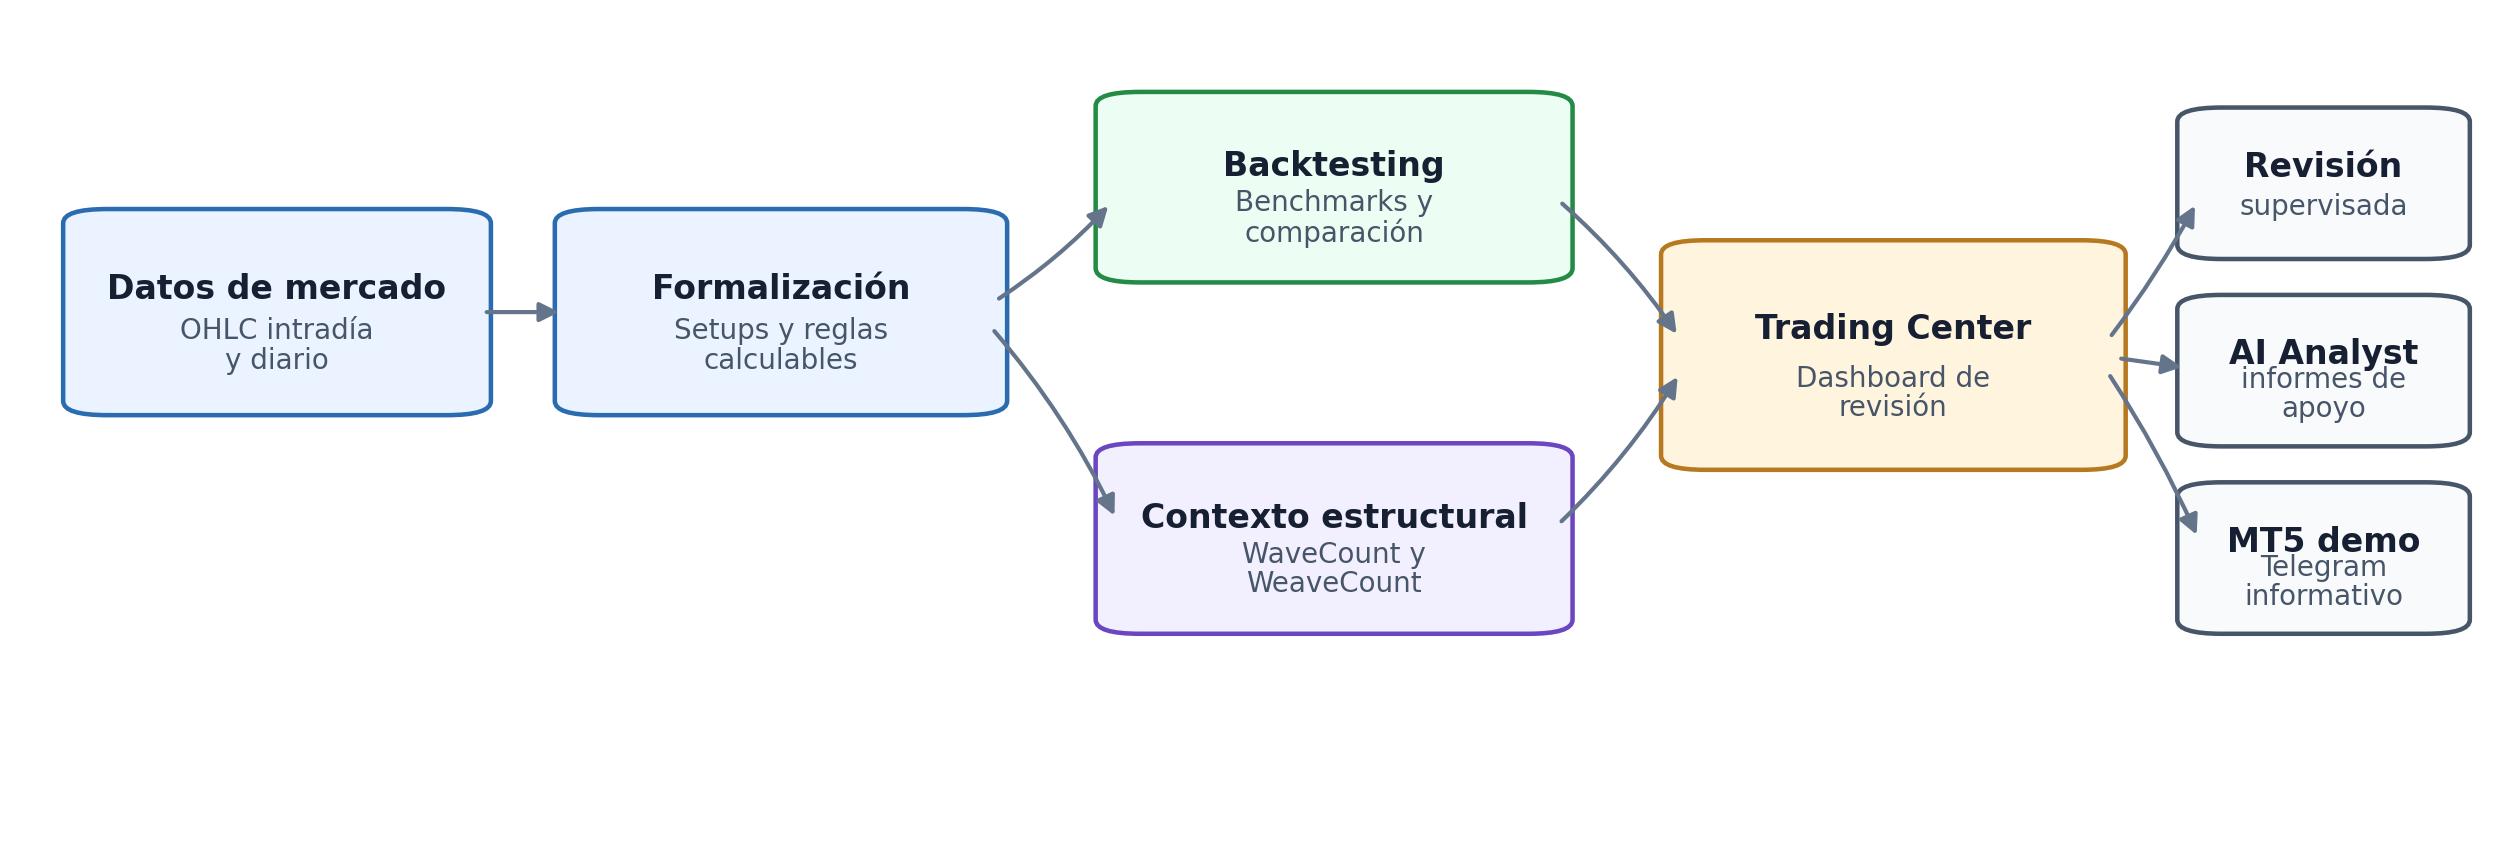
\includegraphics[width=\textwidth]{figs/canonicas/introduccion/flujo_general_tfg_canonico.png}
\caption[Flujo general del trabajo desarrollado]{Flujo general del trabajo desarrollado. La figura resume el paso desde
datos y reglas formalizadas hacia evaluaci\'on hist\'orica, contexto estructural
y revisi\'on supervisada mediante el Trading Center. AI Analyst, MT5 demo y
Telegram aparecen como capas de apoyo y observabilidad, no como mecanismos de
operaci\'on real aut\'onoma.}
\label{fig:flujo-general-tfg}
\end{figure}

\section{Alcance y organizaci\'on de la memoria}

El alcance del trabajo se limita a la formalizaci\'on, evaluaci\'on y presentaci\'on
de un sistema de apoyo al an\'alisis de estrategias de trading. Se incluyen la
preparaci\'on de datos, la definici\'on de reglas, la ejecuci\'on de pruebas
hist\'oricas, el an\'alisis estructural, el desarrollo del dashboard y las capas
auxiliares necesarias para documentar el flujo de revisi\'on. Quedan fuera del
alcance la recomendaci\'on financiera, la operaci\'on en cuenta real, la
automatizaci\'on aut\'onoma en producci\'on, la operaci\'on continua como servicio,
la gesti\'on integral de cartera y la afirmaci\'on de rentabilidad futura.

La memoria se organiza de forma progresiva. Este primer cap\'itulo introduce la
motivaci\'on, el problema, los objetivos y el alcance del trabajo. El Cap\'itulo 2
describe los datos, la metodolog\'ia y la arquitectura del sistema. El
Cap\'itulo 3 presenta y discute los resultados. El Cap\'itulo 4 recoge las
conclusiones, las limitaciones y el trabajo futuro.
